%# -*- coding: utf-8-unix -*-
%%==================================================
%% thesis.tex
%%==================================================

% 双面打印
\documentclass[doctor, adobefonts, openright, twoside, cs4size]{sjtuthesis}
% \documentclass[bachelor, adobefonts, openany, oneside, cs4size, submit]{sjtuthesis} 
% \documentclass[master, adobefonts, review]{sjtuthesis} 
% \documentclass[%
%   bachelor|master|doctor,	% 必选项
%   adobefonts|winfonts,  	% 只测试了adobefonts,请使用adobefonts
%   oneside|twoside,		% 单面打印,双面打印(奇偶页交换页边距,默认)
%   openany|openright, 		% 可以在奇数或者偶数页开新章|只在奇数页开新章(默认)
%   cs4size|c5size, 		% 正文字号:小四、五号(默认)
%   review,	 		% 盲审论文,隐去作者姓名、学号、导师姓名、致谢、发表论文和参与的项目
%   submit			% 定稿提交的论文,插入签名扫描版的原创性声明、授权声明 
% ]

% 逐个导入参考文献数据库
\addbibresource{bib/thesis.bib}
% \addbibresource{bib/chap2.bib}

\begin{document}

%% 无编号内容:中英文论文封面、授权页
%# -*- coding: utf-8-unix -*-
\title{上海交通大学学位论文 \LaTeX 模板示例文档}
\author{某\quad{}某}
\advisor{某某教授}
% \coadvisor{某某教授}
\defenddate{2014年12月17日}
\school{上海交通大学}
\institute{某某系}
\studentnumber{0010900990}
\major{某某专业}

\englishtitle{A Sample Document for \LaTeX-basedd SJTU Thesis Template}
\englishauthor{\textsc{Mo Mo}}
\englishadvisor{Prof. \textsc{Mou Mou}}
% \englishcoadvisor{Prof. \textsc{Uom Uom}}
\englishschool{Shanghai Jiao Tong University}
\englishinstitute{\textsc{Depart of XXX, School of XXX} \\
  \textsc{Shanghai Jiao Tong University} \\
  \textsc{Shanghai, P.R.China}}
\englishmajor{A Very Important Major}
\englishdate{Dec. 17th, 2014}


\maketitle

\makeenglishtitle

\makeatletter
\ifsjtu@submit\relax
	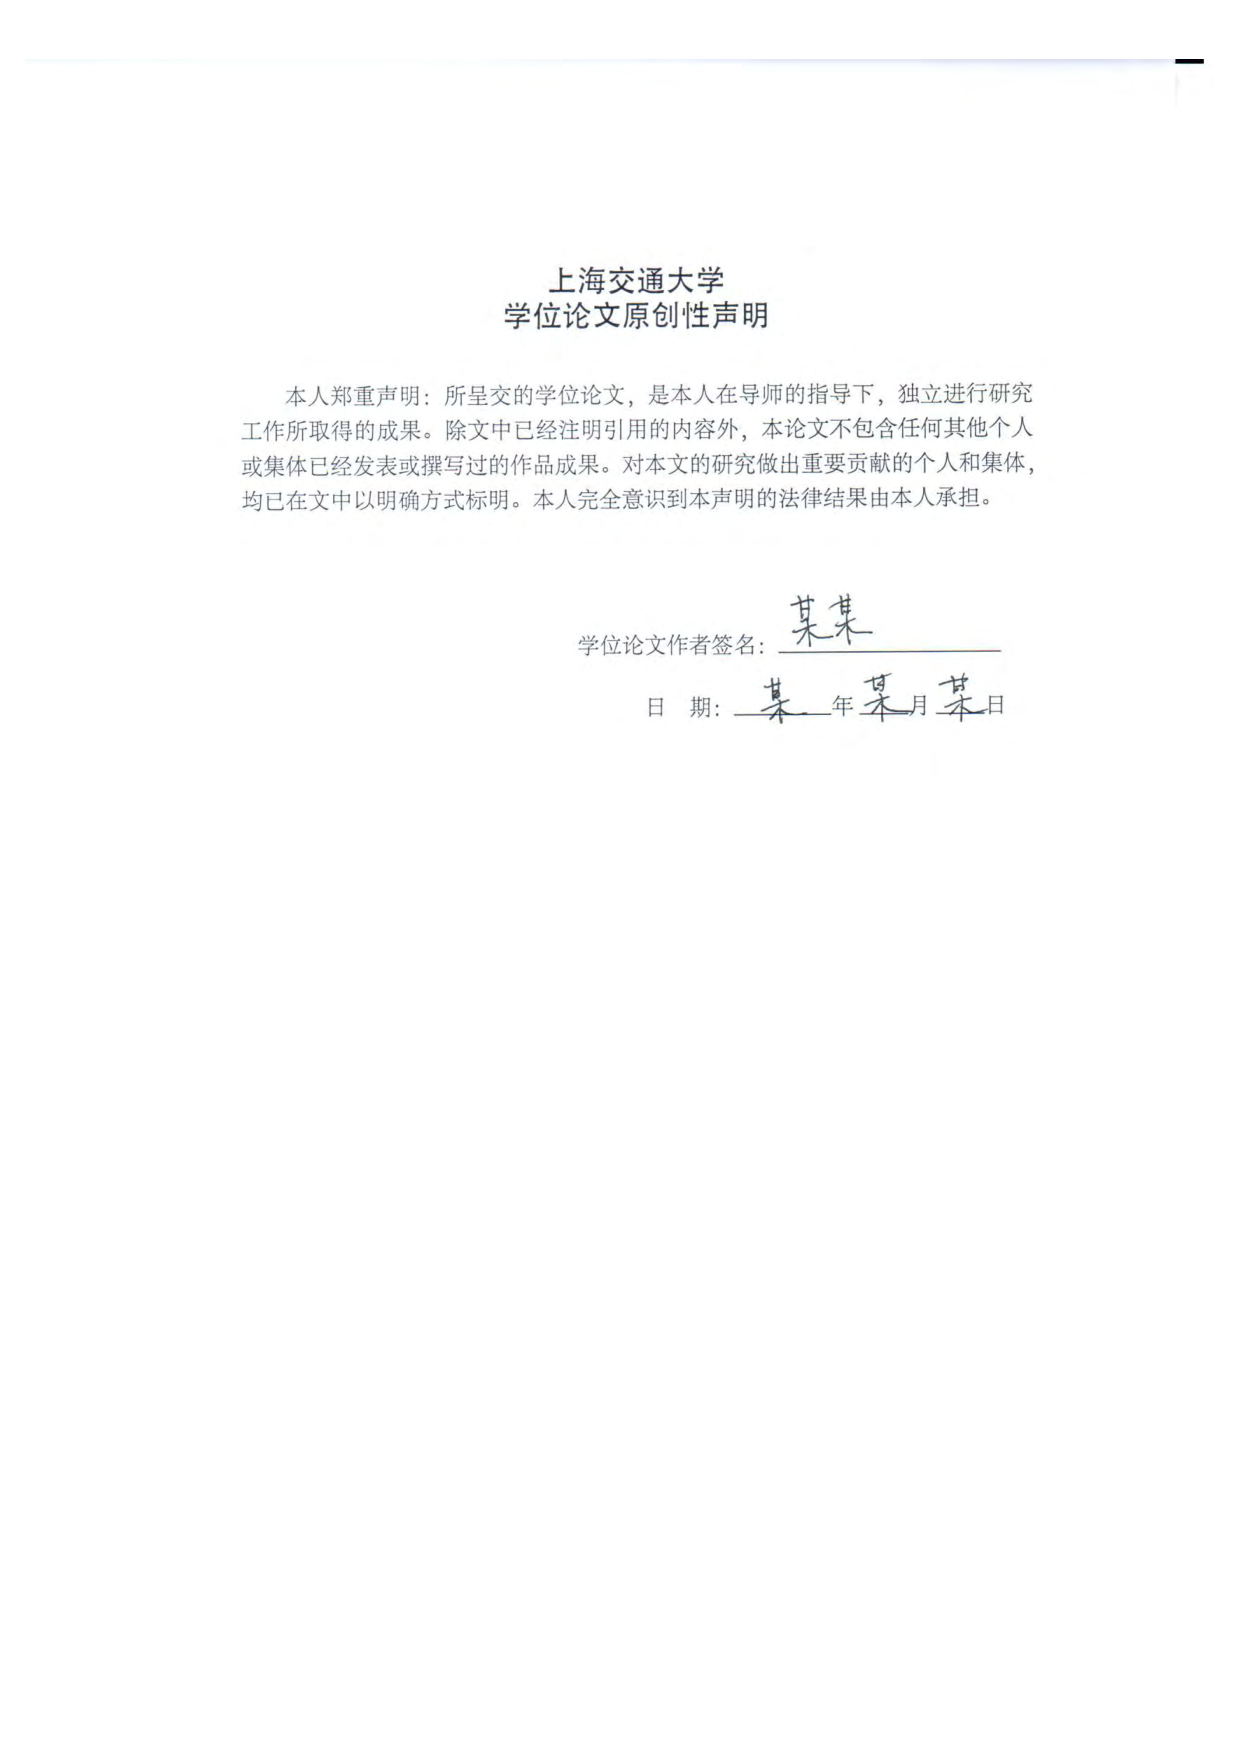
\includepdf{pdf/original.pdf}
	\cleardoublepage
	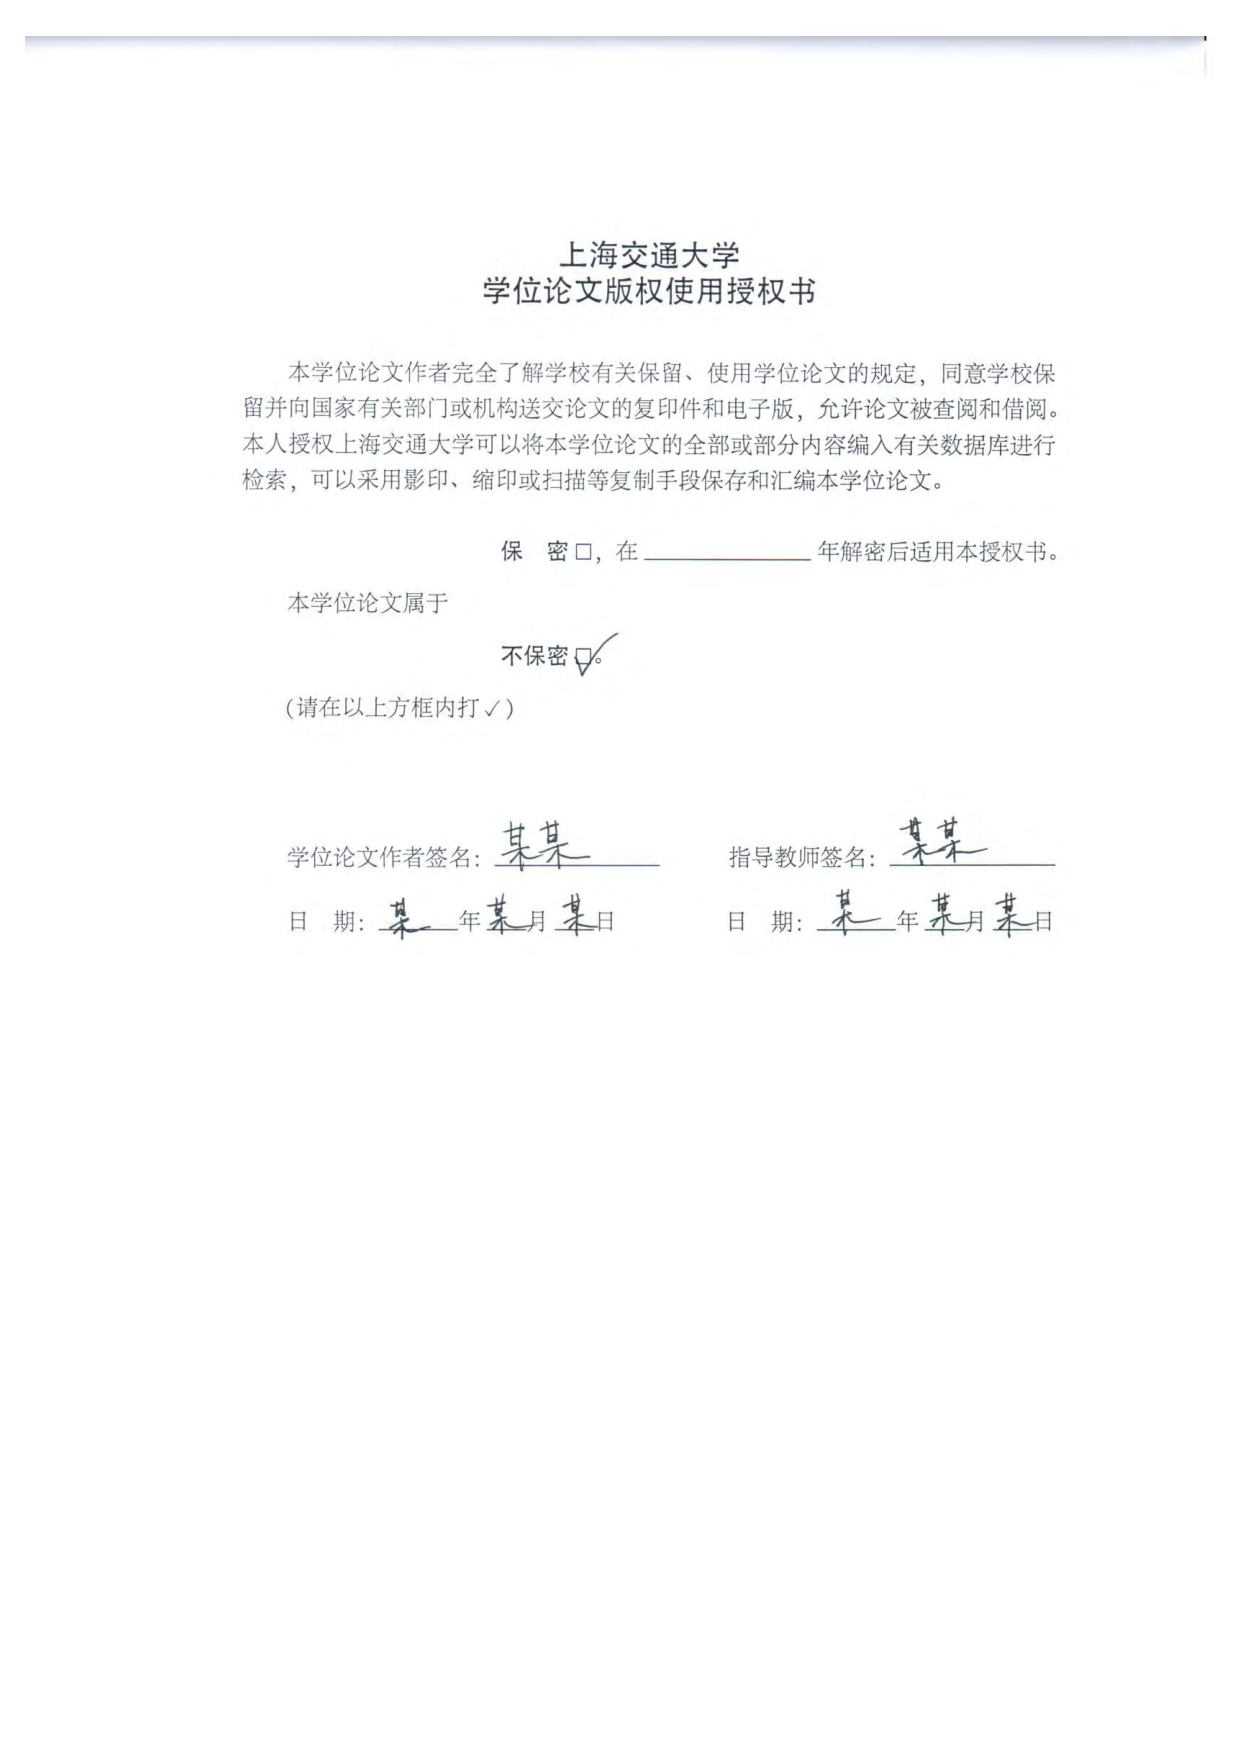
\includepdf{pdf/authorization.pdf}
	\cleardoublepage
\else
	\makeDeclareOriginal
	\makeDeclareAuthorization
\fi
\makeatother


\frontmatter 	% 使用罗马数字对前言编号

%% 摘要
\pagestyle{main}
%%==================================================
%% abstract.tex for SJTU Master Thesis
%%==================================================

\begin{abstract}

上海交通大学是我国历史最悠久的高等学府之一,是教育部直属、教育部与上海市共建的全国重点大学,是国家 “七五”、“八五”重点建设和“211工程”、“985工程”的首批建设高校。经过115年的不懈努力,上海交通大学已经成为一所“综合性、研究型、国际化”的国内一流、国际知名大学,并正在向世界一流大学稳步迈进。 

十九世纪末,甲午战败,民族危难。中国近代著名实业家、教育家盛宣怀和一批有识之士秉持“自强首在储才,储才必先兴学”的信念,于1896年在上海创办了交通大学的前身——南洋公学。建校伊始,学校即坚持“求实学,务实业”的宗旨,以培养“第一等人才”为教育目标,精勤进取,笃行不倦,在二十世纪二三十年代已成为国内著名的高等学府,被誉为“东方MIT”。抗战时期,广大师生历尽艰难,移转租界,内迁重庆,坚持办学,不少学生投笔从戎,浴血沙场。解放前夕,广大师生积极投身民主革命,学校被誉为“民主堡垒”。

新中国成立初期,为配合国家经济建设的需要,学校调整出相当一部分优势专业、师资设备,支持国内兄弟院校的发展。五十年代中期,学校又响应国家建设大西北的号召,根据国务院决定,部分迁往西安,分为交通大学上海部分和西安部分。1959年3月两部分同时被列为全国重点大学,7月经国务院批准分别独立建制,交通大学上海部分启用“上海交通大学”校名。历经西迁、两地办学、独立办学等变迁,为构建新中国的高等教育体系,促进社会主义建设做出了重要贡献。六七十年代,学校先后归属国防科工委和六机部领导,积极投身国防人才培养和国防科研,为“两弹一星”和国防现代化做出了巨大贡献。

改革开放以来,学校以“敢为天下先”的精神,大胆推进改革:率先组成教授代表团访问美国,率先实行校内管理体制改革,率先接受海外友人巨资捐赠等,有力地推动了学校的教学科研改革。1984年,邓小平同志亲切接见了学校领导和师生代表,对学校的各项改革给予了充分肯定。在国家和上海市的大力支持下,学校以“上水平、创一流”为目标,以学科建设为龙头,先后恢复和兴建了理科、管理学科、生命学科、法学和人文学科等。1999年,上海农学院并入;2005年,与上海第二医科大学强强合并。至此,学校完成了综合性大学的学科布局。近年来,通过国家“985工程”和“211工程”的建设,学校高层次人才日渐汇聚,科研实力快速提升,实现了向研究型大学的转变。与此同时,学校通过与美国密西根大学等世界一流大学的合作办学,实施国际化战略取得重要突破。1985年开始闵行校区建设,历经20多年,已基本建设成设施完善,环境优美的现代化大学校园,并已完成了办学重心向闵行校区的转移。学校现有徐汇、闵行、法华、七宝和重庆南路(卢湾)5个校区,总占地面积4840亩。通过一系列的改革和建设,学校的各项办学指标大幅度上升,实现了跨越式发展,整体实力显著增强,为建设世界一流大学奠定了坚实的基础。

交通大学始终把人才培养作为办学的根本任务。一百多年来,学校为国家和社会培养了20余万各类优秀人才,包括一批杰出的政治家、科学家、社会活动家、实业家、工程技术专家和医学专家,如江泽民、陆定一、丁关根、汪道涵、钱学森、吴文俊、徐光宪、张光斗、黄炎培、邵力子、李叔同、蔡锷、邹韬奋、陈敏章、王振义、陈竺等。在中国科学院、中国工程院院士中,有200余位交大校友;在国家23位“两弹一星”功臣中,有6位交大校友;在18位国家最高科学技术奖获得者中,有3位来自交大。交大创造了中国近现代发展史上的诸多“第一”:中国最早的内燃机、最早的电机、最早的中文打字机等;新中国第一艘万吨轮、第一艘核潜艇、第一艘气垫船、第一艘水翼艇、自主设计的第一代战斗机、第一枚运载火箭、第一颗人造卫星、第一例心脏二尖瓣分离术、第一例成功移植同种原位肝手术、第一例成功抢救大面积烧伤病人手术等,都凝聚着交大师生和校友的心血智慧。改革开放以来,一批年轻的校友已在世界各地、各行各业崭露头角。

截至2011年12月31日,学校共有24个学院/直属系(另有继续教育学院、技术学院和国际教育学院),19个直属单位,12家附属医院,全日制本科生16802人、研究生24495人(其中博士研究生5059人);有专任教师2979名,其中教授835名;中国科学院院士15名,中国工程院院士20名,中组部“千人计划”49名,“长江学者”95名,国家杰出青年基金获得者80名,国家重点基础研究发展计划(973计划)首席科学家24名,国家重大科学研究计划首席科学家9名,国家基金委创新研究群体6个,教育部创新团队17个。

学校现有本科专业68个,涵盖经济学、法学、文学、理学、工学、农学、医学、管理学和艺术等九个学科门类;拥有国家级教学及人才培养基地7个,国家级校外实践教育基地5个,国家级实验教学示范中心5个,上海市实验教学示范中心4个;有国家级教学团队8个,上海市教学团队15个;有国家级教学名师7人,上海市教学名师35人;有国家级精品课程46门,上海市精品课程117门;有国家级双语示范课程7门;2001、2005和2009年,作为第一完成单位,共获得国家级教学成果37项、上海市教学成果157项。

\keywords{\large 上海交大 \quad 饮水思源 \quad 爱国荣校}
\end{abstract}

\begin{englishabstract}

An imperial edict issued in 1896 by Emperor Guangxu, established Nanyang Public School in Shanghai. The normal school, school of foreign studies, middle school and a high school were established. Sheng Xuanhuai, the person responsible for proposing the idea to the emperor, became the first president and is regarded as the founder of the university.

During the 1930s, the university gained a reputation of nurturing top engineers. After the foundation of People's Republic, some faculties were transferred to other universities. A significant amount of its faculty were sent in 1956, by the national government, to Xi'an to help build up Xi'an Jiao Tong University in western China. Afterwards, the school was officially renamed Shanghai Jiao Tong University.

Since the reform and opening up policy in China, SJTU has taken the lead in management reform of institutions for higher education, regaining its vigor and vitality with an unprecedented momentum of growth. SJTU includes five beautiful campuses, Xuhui, Minhang, Luwan Qibao, and Fahua, taking up an area of about 3,225,833 m2. A number of disciplines have been advancing towards the top echelon internationally, and a batch of burgeoning branches of learning have taken an important position domestically.

Today SJTU has 31 schools (departments), 63 undergraduate programs, 250 masters-degree programs, 203 Ph.D. programs, 28 post-doctorate programs, and 11 state key laboratories and national engineering research centers.

SJTU boasts a large number of famous scientists and professors, including 35 academics of the Academy of Sciences and Academy of Engineering, 95 accredited professors and chair professors of the "Cheung Kong Scholars Program" and more than 2,000 professors and associate professors.

Its total enrollment of students amounts to 35,929, of which 1,564 are international students. There are 16,802 undergraduates, and 17,563 masters and Ph.D. candidates. After more than a century of operation, Jiao Tong University has inherited the old tradition of "high starting points, solid foundation, strict requirements and extensive practice." Students from SJTU have won top prizes in various competitions, including ACM International Collegiate Programming Contest, International Mathematical Contest in Modeling and Electronics Design Contests. Famous alumni include Jiang Zemin, Lu Dingyi, Ding Guangen, Wang Daohan, Qian Xuesen, Wu Wenjun, Zou Taofen, Mao Yisheng, Cai Er, Huang Yanpei, Shao Lizi, Wang An and many more. More than 200 of the academics of the Chinese Academy of Sciences and Chinese Academy of Engineering are alumni of Jiao Tong University.

\englishkeywords{\large SJTU, master thesis, XeTeX/LaTeX template}
\end{englishabstract}



%% 目录、插图目录、表格目录
\tableofcontents
\listoffigures
\addcontentsline{toc}{chapter}{\listfigurename} %将插图目录加入全文目录
\listoftables
\addcontentsline{toc}{chapter}{\listtablename}  %将表格目录加入全文目录
% \listofalgorithms
% \addcontentsline{toc}{chapter}{代码索引}  %将表格目录加入全文目录

%# -*- coding: utf-8-unix -*-
\chapter{主要符号对照表}
\label{chap:symb}

\begin{longtable}{rl}
$\epsilon$     & 介电常数 \\
 $\mu$ 		& 磁导率 \\
 $\epsilon$     & 介电常数 \\
 $\mu$ 		& 磁导率 \\
 $\epsilon$     & 介电常数 \\
 $\mu$ 		& 磁导率 \\
 $\epsilon$ 	& 介电常数 \\
 $\mu$ 		& 磁导率 \\
 $\epsilon$     & 介电常数 \\
 $\mu$ 		& 磁导率 \\
 $\epsilon$     & 介电常数 \\
 $\mu$ 		& 磁导率 \\
 $\epsilon$     & 介电常数 \\
 $\mu$ 		& 磁导率 \\
 $\epsilon$ 	& 介电常数 \\
 $\mu$ 		& 磁导率 \\
 $\epsilon$     & 介电常数 \\
 $\mu$ 		& 磁导率 \\
 $\epsilon$     & 介电常数 \\
 $\mu$ 		& 磁导率 \\
 $\epsilon$     & 介电常数 \\
 $\mu$ 		& 磁导率 \\
 $\epsilon$ 	& 介电常数 \\
 $\mu$ 		& 磁导率 \\
 $\epsilon$     & 介电常数 \\
 $\mu$ 		& 磁导率 \\
 $\epsilon$     & 介电常数 \\
 $\mu$ 		& 磁导率 \\
 $\epsilon$     & 介电常数 \\
 $\mu$ 		& 磁导率 \\
 $\epsilon$ 	& 介电常数 \\
 $\mu$ 		& 磁导率 \\
 $\epsilon$     & 介电常数 \\
 $\mu$ 		& 磁导率 \\
 $\epsilon$     & 介电常数 \\
 $\mu$ 		& 磁导率 \\
 $\epsilon$     & 介电常数 \\
 $\mu$ 		& 磁导率 \\
 $\epsilon$ 	& 介电常数 \\
 $\mu$ 		& 磁导率 \\
 $\epsilon$     & 介电常数 \\
 $\mu$ 		& 磁导率 \\
 $\epsilon$     & 介电常数 \\
 $\mu$ 		& 磁导率 \\
 $\epsilon$     & 介电常数 \\
 $\mu$ 		& 磁导率 \\
 $\epsilon$ 	& 介电常数 \\
 $\mu$ 		& 磁导率 \\
 $\epsilon$     & 介电常数 \\
 $\mu$ 		& 磁导率 \\
 $\epsilon$     & 介电常数 \\
 $\mu$ 		& 磁导率 \\
 $\epsilon$     & 介电常数 \\
 $\mu$ 		& 磁导率 \\
\end{longtable}
 % 主要符号、缩略词对照表

\mainmatter	% 使用阿拉伯数字对正文编号

%% 正文内容
\pagestyle{main}
%%==================================================
%% chapter01.tex for SJTU Master Thesis
%%==================================================

%\bibliographystyle{sjtu2}%[此处用于每章都生产参考文献]
\chapter{这是什么}
\label{chap:what}

这是上海交通大学(非官方)学位论文 \LaTeX 模板,当前版本是 \version 。

最早的一版学位模板是一位热心的物理系同学制作的。
那份模板参考了自动化所学位论文模板,使用了CASthesis.cls文档类,中文字符处理则采用当时最为流行的 \CJKLaTeX 方案。
我根据交大研究生院对学位论文的要求
\footnote{\url{http://www.gs.sjtu.edu.cn/policy/fileShow.ahtml?id=130}}
,结合少量个人审美喜好,完成了一份基本可用的交大 \LaTeX 学位论文模板。
但是,搭建一个 \CJKLaTeX 环境并不简单,单单在Linux下配置环境和添加中文字体,就足够让新手打退堂鼓。
在William Wang的建议下,我开始着手把模板向 \XeTeX 引擎移植。
他完成了最初的移植,多亏了他出色的工作,后续的改善工作也得以顺利进行。

随着我对 \LaTeX 系统认知增加,我又断断续续做了一些完善模板的工作,在原有硕士学位论文模板的基础上完成了交大学士和博士学位论文模板。

现在,交大学位论文模板SJTUTHesis代码在github
\footnote{\url{https://github.com/weijianwen/SJTUThesis}}
上维护。
你可以\href{https://github.com/weijianwen/SJTUThesis/issues}{在github上开issue}
、或者在\href{https://bbs.sjtu.edu.cn/bbsdoc?board=TeX_LaTeX}{水源LaTeX版}发帖来反映遇到的问题。

\section{使用模板}

\subsection{准备工作}
\label{sec:requirements}

要使用这个模板撰写学位论文,需要在\emph{TeX系统}、\emph{中英文字体}、\emph{TeX技能}上有所准备。

\begin{itemize}[noitemsep,topsep=0pt,parsep=0pt,partopsep=0pt]
	\item {\TeX}系统:所使用的{\TeX}系统要支持 \XeTeX 引擎,以2014年以后发布的\emph{完整}CTeX、TeXLive、MacTeX发行版为佳。
	\item 中英文字体:操作系统中需要安装\footnote{在Windows、Mac OS X 以及 Linux 上安装额外的字体,可以参考\href{https://www.searchfreefonts.com/articles/how-to-install-fonts.htm}{“How to install fonts?”}。
}TeX Gyre Termes字体\footnote{\url{http://www.gust.org.pl/projects/e-foundry/tex-gyre/termes}}和四款Adobe中文字体
\footnote{请从合法渠道获得Adobe字体。}:AdobeSongStd、AdobeKaitiStd、AdobeHeitiStd、AdobeFangsongStd。
	\item TeX技能:尽管提供了对模板的必要说明,但这不是一份“ \LaTeX 入门文档”。在使用前请先通读其他入门文档。
	\item 针对Windows用户的额外需求:学位论文模本默认使用GNUMake在命令提示符下构建,建议从Cygwin\footnote{\url{http://cygwin.com}}安装GNU工具集。
\end{itemize}

\subsection{模板选项}
\label{sec:thesisoption}

sjtuthesis提供了一些常用选项,在thesis.tex在导入sjtuthesis模板类时,可以组合使用。
这些选项包括:

\begin{itemize}[noitemsep,topsep=0pt,parsep=0pt,partopsep=0pt]
\item 学位类型:bachelor(学位)、master(硕士)、doctor(博士),是必选项。
\item 中国字体:adobefonts(Adobe中文字体)、winfonts(使用Windows下的中文字体,改选项未在Linux/Mac下测试)。
\item 正文字号:cs4size(小四)、c5size(五号)。
\item 盲审选项:使用review选项后,论文作者、学号、导师姓名、致谢、发表论文和参与项目将被隐去。
\end{itemize}

\subsection{编译模板}
\label{sec:process}

模板默认使用GNUMake构建,GNUMake将调用latemk工具自动完成模板多轮编译:

\begin{lstlisting}[basicstyle=\small\ttfamily, caption={编译模板}, numbers=none]
make clean thesis.pdf
\end{lstlisting}

若需要生成包含“原创性声明扫描件”的学位论文文档,请将扫描件保存为statement.pdf,然后调用make生成submit.pdf。

\begin{lstlisting}[basicstyle=\small\ttfamily, caption={生成用于提交的学位论文}, numbers=none]
make clean submit.pdf
\end{lstlisting}

编译失败时,可以尝试手动逐次编译,定位故障。

\begin{lstlisting}[basicstyle=\small\ttfamily, caption={手动逐次编译}, numbers=none]
xelatex -no-pdf thesis
biber --debug thesis
xelatex thesis
xelatex thesis
\end{lstlisting}

\subsection{模板文件布局}
\label{sec:layout}

\begin{lstlisting}[basicstyle=\small\ttfamily,caption={模板文件布局},label=layout,float,numbers=none]
├── LICENSE
├── Makefile
├── README.md
├── bib
│   ├── chap1.bib
│   └── chap2.bib
├── bst
│   └── GBT7714-2005NLang.bst
├── figure
│   ├── chap2
│   │   ├── sjtulogo.eps
│   │   ├── sjtulogo.jpg
│   │   ├── sjtulogo.pdf
│   │   └── sjtulogo.png
│   └── sjtubanner.png
├── sjtuthesis.cfg
├── sjtuthesis.cls
├── statement.pdf
├── submit.pdf
├── tex
│   ├── abstract.tex
│   ├── ack.tex
│   ├── app_cjk.tex
│   ├── app_eq.tex
│   ├── app_log.tex
│   ├── chapter01.tex
│   ├── chapter02.tex
│   ├── chapter03.tex
│   ├── conclusion.tex
│   ├── id.tex
│   ├── patents.tex
│   ├── projects.tex
│   ├── pub.tex
│   └── symbol.tex
└── thesis.tex
\end{lstlisting}

本节介绍学位论文模板中木要文件和目录的功能。

\subsubsection{格式控制文件}
\label{sec:format}

格式控制文件控制着论文的表现形式,包括以下几个文件:
sjtuthesis.cfg, sjtuthesis.cls和GBT7714-2005NLang.bst。
其中,“cfg”和“cls”控制论文主体格式,“bst”控制参考文献条目的格式,

\subsubsection{主控文件thesis.tex}
\label{sec:thesistex}

主控文件thesis.tex的作用就是将你分散在多个文件中的内容“整合”成一篇完整的论文。
使用这个模板撰写学位论文时,你的学位论文内容和素材会被“拆散”到各个文件中:
譬如各章正文、各个附录、各章参考文献等等。
在thesis.tex中通过“include”命令将论文的各个部分包含进来,从而形成一篇结构完成的论文。
对模板定制时引入的宏包,建议放在导言区。

\subsubsection{各章源文件tex}
\label{sec:thesisbody}

这一部分是论文的主体,是以“章”为单位划分的,包括:

\begin{itemize}[noitemsep,topsep=0pt,parsep=0pt,partopsep=0pt]
	\item 中英文摘要(abstract.tex)。前言(frontmatter)的其他部分,中英文封面、原创性声明、授权信息在sjtuthesis.cls中定义,不单独分离为tex文件。
不单独弄成文件。
	\item 正文(mainmatter)——学位论文正文的各章内容,源文件是chapter\emph{xxx}.tex。
	\item 附录(app\emph{xx}.tex)、致谢(thuanks.tex)、攻读学位论文期间发表的学术论文目录(pub.tex)、个人简历(resume.tex)组成正文后的部分(backmatter)。
参考文献列表由bibtex插入,不作为一个单独的文件。
\end{itemize}

\subsubsection{图片文件夹figure}
\label{sec:fig}

figure文件夹放置了需要插入文档中的图片文件(支持PNG/JPG/PDF/EPS格式的图片),可以在按照章节划分子目录。
模板文件中使用\verb|\graphicspath|命令定义了图片存储的顶层目录,在插入图片时,顶层目录名“figure”可省略。

\subsubsection{参考文献数据库bib}
\label{sec:bib}

目前参考文件数据库目录只存放一个参考文件数据库thesis.bib。
关于参考文献引用,可参考第\ref{chap:example}章中的例子。


%%==================================================
%% chapter02.tex for SJTU Master Thesis
%% based on CASthesis
%% modified by wei.jianwen@gmail.com
%% Encoding: UTF-8
%%==================================================

\chapter{一些 \LaTeX 排版的例子}
\label{chap:example}

\section{数学排版的例子}
\label{sec:matheq}

\subsection{公式排版}
\label{sec:eqformat}

这里有举一个长公式排版的例子,来自\href{http://www.tex.ac.uk/tex-archive/info/math/voss/mathmode/Mathmode.pdf}{《Math mode》}:

\begin {multline}
  \frac {1}{2}\Delta (f_{ij}f^{ij})=
  2\left (\sum _{i<j}\chi _{ij}(\sigma _{i}-
    \sigma _{j}) ^{2}+ f^{ij}\nabla _{j}\nabla _{i}(\Delta f)+\right .\\
  \left .+\nabla _{k}f_{ij}\nabla ^{k}f^{ij}+
    f^{ij}f^{k}\left [2\nabla _{i}R_{jk}-
      \nabla _{k}R_{ij}\right ]\vphantom {\sum _{i<j}}\right )
\end{multline}

\subsubsection{一个四级标题}
\label{sec:depth4}

这是全文唯一的一个四级标题。在这部分中将演示可伸长符号(箭头、等号的例子)的例子,以及如何在可伸长的符号上标注。在\href{http://www.ctex.org/CTeXFAQ/files.xml?action=download&file=ctex-faq.pdf}{《CTeX常见问题集》}中也由类似的介绍。
首先需要在diss.tex导言区引入如下的内容:

\begin{lstlisting}[language={TeX}, caption={插入导言区的内容}]
  \makeatletter
  \def\ExtendSymbol#1#2#3#4#5{\ext@arrow 0099{\arrowfill@#1#2#3}{#4}{#5}}
  \def\RightExtendSymbol#1#2#3#4#5{\ext@arrow 0359{\arrowfill@#1#2#3}{#4}{#5}}
  \def\LeftExtendSymbol#1#2#3#4#5{\ext@arrow 6095{\arrowfill@#1#2#3}{#4}{#5}}
  \makeatother
  
  \newcommand\myRightarrow[2][]{\RightExtendSymbol{=}{=}{\Rightarrow}{#1}{#2}}
  \newcommand\myLeftarrow[2][]{\LeftExtendSymbol{\Leftarrow}{=}{=}{#1}{#2}}
  \newcommand\myBioarrow[2][]{\ExtendSymbol{\Leftarrow}{=}{\Rightarrow}{#1}{#2}}
  \newcommand\myLongEqual[2][]{\ExtendSymbol{=}{=}{=}{#1}{#2}}
\end{lstlisting}

然后,在正文插入如代码\ref{mathextend}所示的内容。效果如下:

\begin{lstlisting}[language={TeX}, caption={可伸长的符号},label=mathextend,float]
  \begin{eqnarray}
    f(x) & \myBioarrow{A=B}  & B \\
    & \myLongEqual{A=B} & B \\
    & \myLeftarrow[A=B^2]{B=A^2} & B \nonumber \\
    & \myRightarrow{B^2=A^2} & B
  \end{eqnarray}
\end{lstlisting}

\begin{displaymath}
    A \xleftarrow{n=0} B \xrightarrow[LongLongLongLong]{n>0} C 
\end{displaymath}

\begin{eqnarray}
  f(x) & \myBioarrow{A=B}  & B \\
  & \myLongEqual{A=B} & B \\
  & \myLeftarrow[A=B^2]{B=A^2} & B \nonumber \\
  & \myRightarrow{B^2=A^2} & B
\end{eqnarray}

又如:

\begin{align}
  \label{eq:none}
  & I(X_3;X_4)-I(X_3;X_4|X_1)-I(X_3;X_4|X_2) \nonumber \\
  \myLongEqual{a)}\, & [I(X_3;X_4)-I(X_3;X_4|X_1)]-I(X_3;X_4|\tilde{X}_2) \\
  \myLongEqual[\rule{0.28cm}{0cm}]{}\, & I(X_1;X_3;X_4)-I(X_3;X_4|\tilde{X}_2)
\end{align}


\subsection{定理环境}

模板中定义了丰富的定理环境
algo(算法),thm(定理),lem(引理),prop(命题),cor(推论),defn(定义),conj(猜想),exmp(例),rem(注),case(情形),
bthm(断言定理),blem(断言引理),bprop(断言命题),bcor(断言推论)。
amsmath还提供了一个proof(证明)的环境。
这里举一个``定理''和``证明''的例子。
\begin{thm}[留数定理]
\label{thm:res}
  假设$U$是复平面上的一个单连通开子集,$a_1,\ldots,a_n$是复平面上有限个点,$f$是定义在$U\backslash \{a_1,\ldots,a_n\}$上的全纯函数,
  如果$\gamma$是一条把$a_1,\ldots,a_n$包围起来的可求长曲线,但不经过任何一个$a_k$,并且其起点与终点重合,那么:

  \begin{equation}
    \label{eq:res}
    \ointop_{\gamma}f(z)\,\mathrm{d}z = 2\uppi\mathbf{i}\sum^n_{k=1}\mathrm{I}(\gamma,a_k)\mathrm{Res}(f,a_k)
  \end{equation}

  如果$\gamma$是若尔当曲线,那么$\mathrm{I}(\gamma, a_k)=1$,因此:

  \begin{equation}
    \label{eq:resthm}
    \ointop_{\gamma}f(z)\,\mathrm{d}z = 2\uppi\mathbf{i}\sum^n_{k=1}\mathrm{Res}(f,a_k)
  \end{equation}

      % \oint_\gamma f(z)\, dz = 2\pi i \sum_{k=1}^n \mathrm{Res}(f, a_k ). 

  在这里,$\mathrm{Res}(f, a_k)$表示$f$在点$a_k$的留数,$\mathrm{I}(\gamma,a_k)$表示$\gamma$关于点$a_k$的卷绕数。
  卷绕数是一个整数,它描述了曲线$\gamma$绕过点$a_k$的次数。如果$\gamma$依逆时针方向绕着$a_k$移动,卷绕数就是一个正数,
  如果$\gamma$根本不绕过$a_k$,卷绕数就是零。

  定理\ref{thm:res}的证明。
  
  \begin{proof}
    首先,由……

    其次,……

    所以……
  \end{proof}
\end{thm}

上面的公式例子中,有一些细节希望大家注意。微分号d应该使用``直立体'',也就是用mathrm包围起来。
并且,微分号和被积函数之间应该有一段小间隔,可以插入\verb+\,+得到。
斜体的$d$通常只作为一般变量。
i,j作为虚数单位时,也应该使用``直立体'',为了明显,还加上了粗体,例如\verb+\mathbf{i}+。斜体$i,j$通常用作表示``序号''。
其他字母在表示常量时,也推荐使用``直立体'',譬如,圆周率$\uppi$(需要upgreek宏包),自然对数的底$\mathrm{e}$。
不过,我个人觉得斜体的$e$和$\pi$很潇洒,在不至于引起混淆的情况下,我也用这两个字母的斜体表示对应的常量。


\section{向文档中插入图像}
\label{sec:insertimage}

\subsection{支持的图片格式}
\label{sec:imageformat}

\XeTeX 可以很方便地插入PDF、EPS、PNG、JPG格式的图片。

插入PNG/JPG的例子如\ref{fig:SRR}所示。
这两个水平并列放置的图共享一个``图标题''(table caption),没有各自的小标题。

\begin{figure}[!htp]
  \centering
  
\includegraphics[width=0.3\textwidth]{chap2/testpng}
  \hspace{1cm}
  
\includegraphics[width=0.3\textwidth]{chap2/testjpg}
  \bicaption[fig:SRR]{这里将出现在插图索引中}{中文题图}{Fig}{English caption}
\end{figure}

这里还有插入eps图像和pdf图像的例子,如图\ref{fig:pdfeps}。这里将EPS和PDF图片作为子图插入,每个子图有自己的小标题。并列子图的功能是使用subfigure宏包提供的。

\begin{figure}
  \centering
  \subfigure[EPS Figure]{
    \label{fig:epspdf:a} %% label for first subfigure
    \includegraphics[width=0.3\textwidth]{chap2/testeps}}
  \hspace{1in}
  \subfigure[PDF Figure]{
    \label{fig:epspdf:b} %% label for second subfigure
    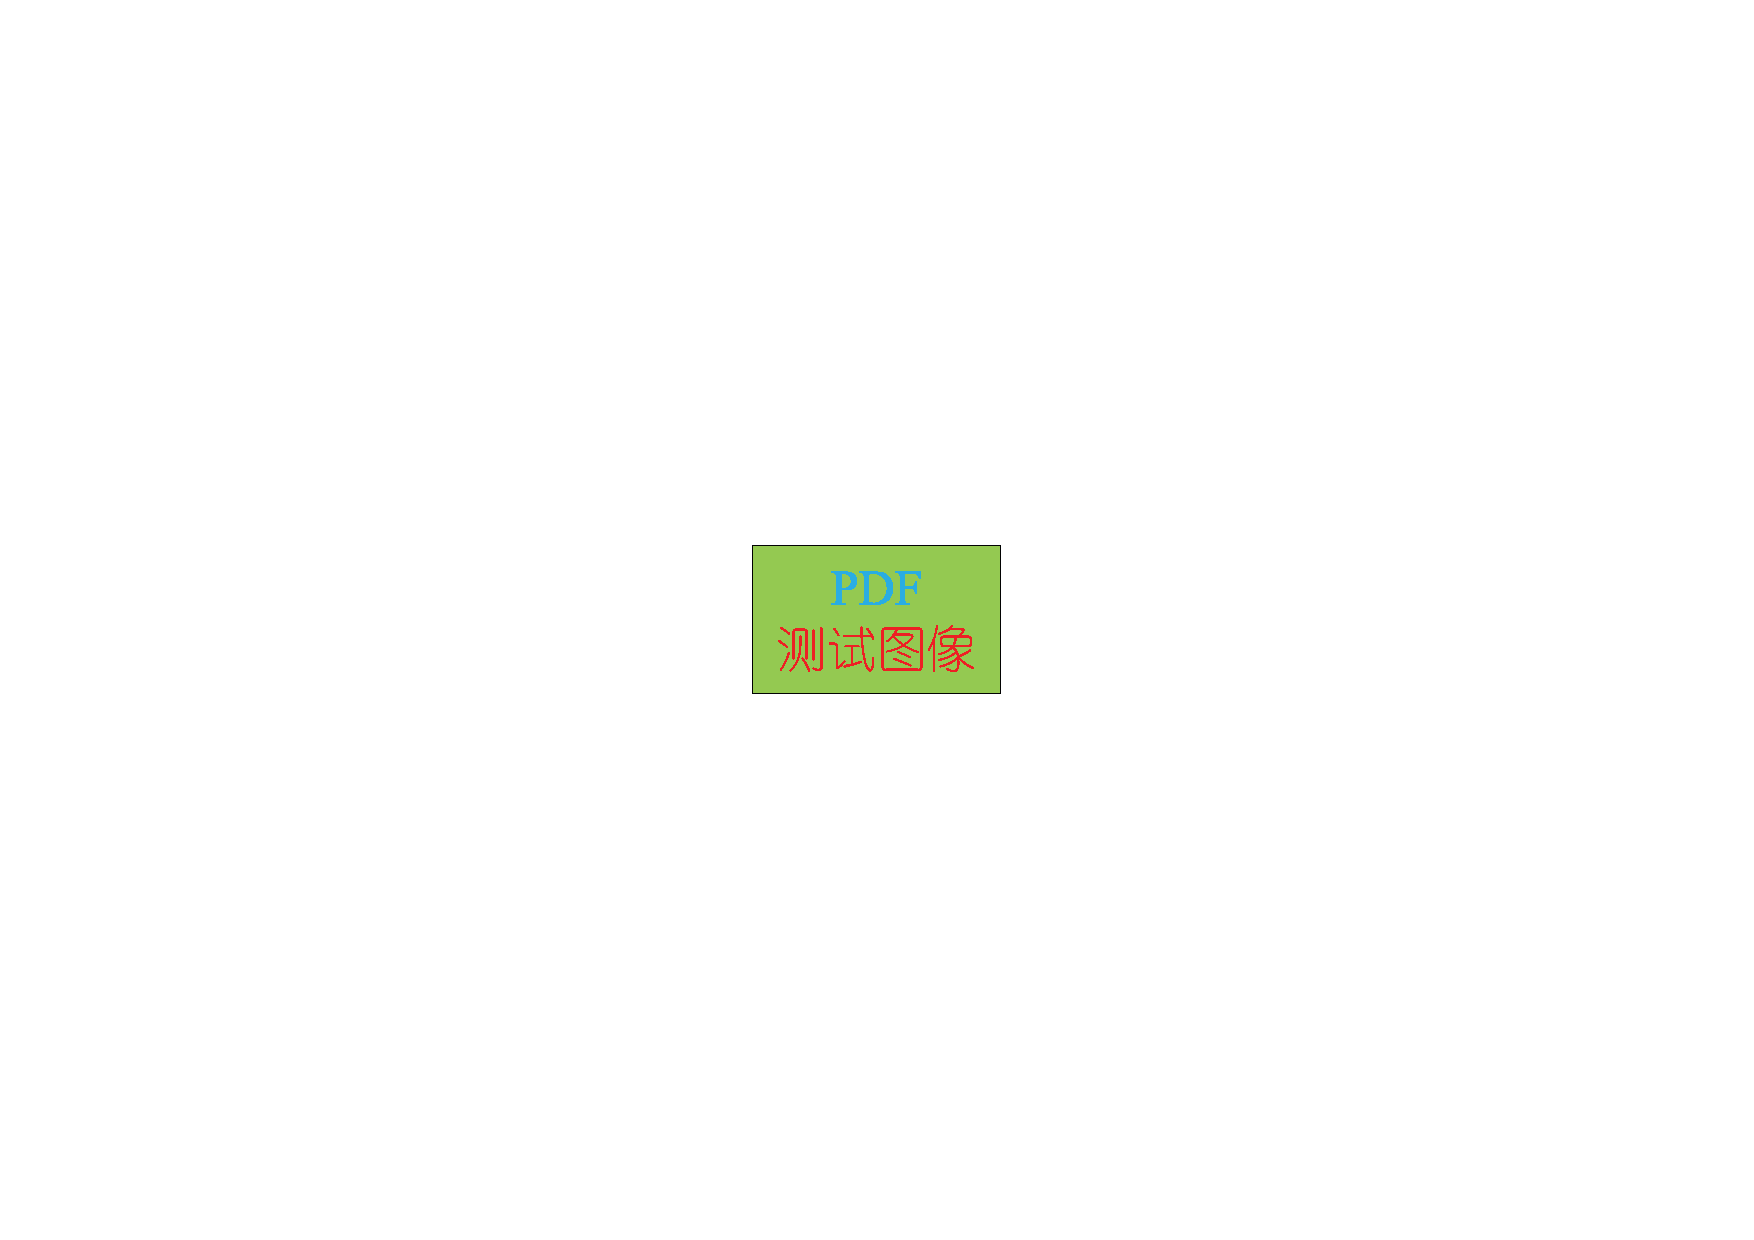
\includegraphics[angle=-90,origin=br,width=0.3\textwidth]{chap2/testpdf.pdf}}
  \bicaption[fig:pdfeps]{插入eps图像和pdf图像}{插入eps和pdf的例子}{Fig}{An EPS and PDF demo}
\end{figure}

更多关于 \LaTeX 插图的例子可以参考\href{http://www.cs.duke.edu/junhu/Graphics3.pdf}{《\LaTeX 插图指南》}。

\subsection{长标题的换行}
\label{sec:longcaption}

图\ref{fig:longcaptionbad}和图\ref{fig:longcaptiongood}都有比较长图标题,通过对比发现,图\ref{fig:longcaptiongood}的换行效果更好一些。
其中使用了minipage环境来限制整个浮动题的宽度。

\begin{figure}[!htp]
 \centering
 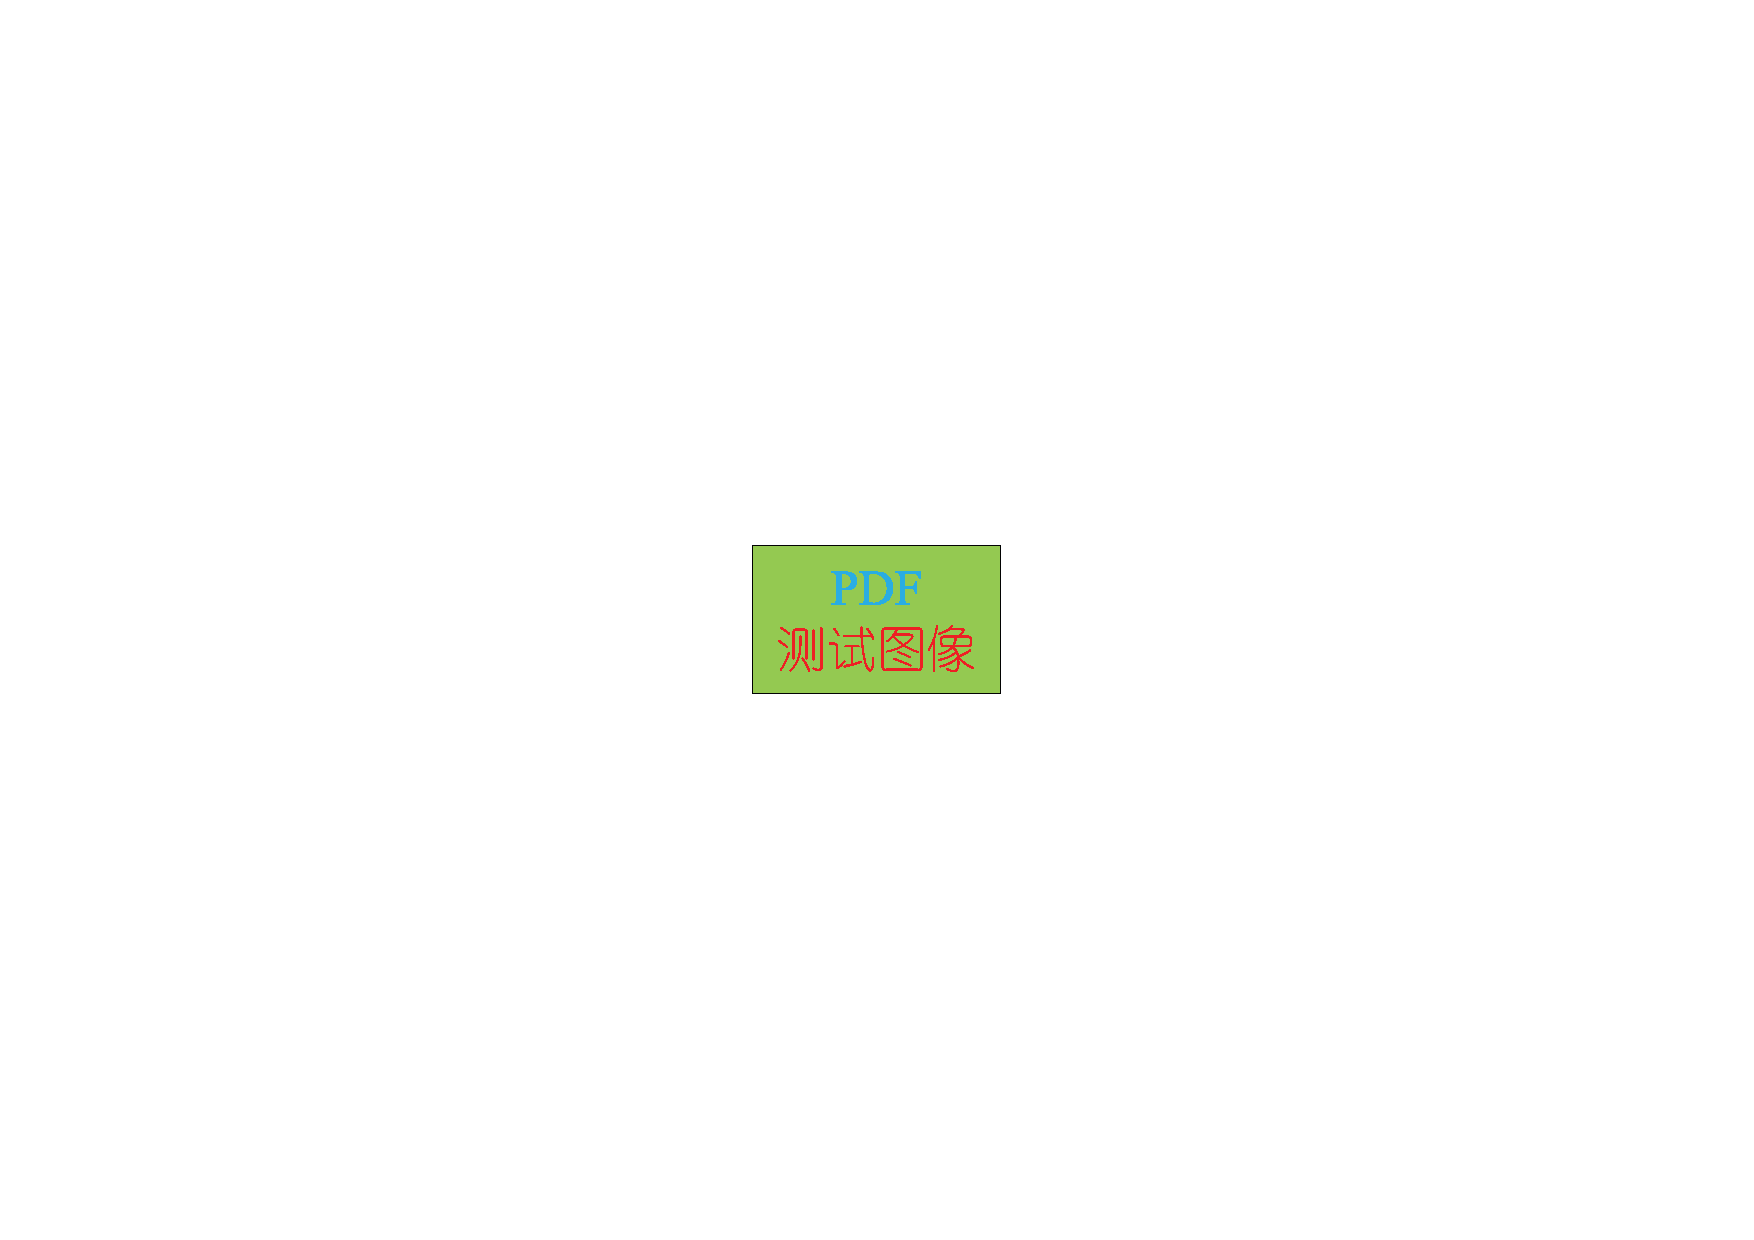
\includegraphics[angle=-90,origin=br,width=4cm]{chap2/testpdf.pdf}
 \bicaption[fig:longcaptionbad]{这里将出现在插图索引}{海交通大学是我国历史最悠久的高等学府之一,是教育部直属、教育部与上海市共建的全国重点大学.}{Fig}{Where there is a will, there is a way.}
\end{figure}


  \begin{figure}[!hbp]
    \centering
    \begin{minipage}[b]{0.6\textwidth}
      \captionstyle{\centering}
      \centering
      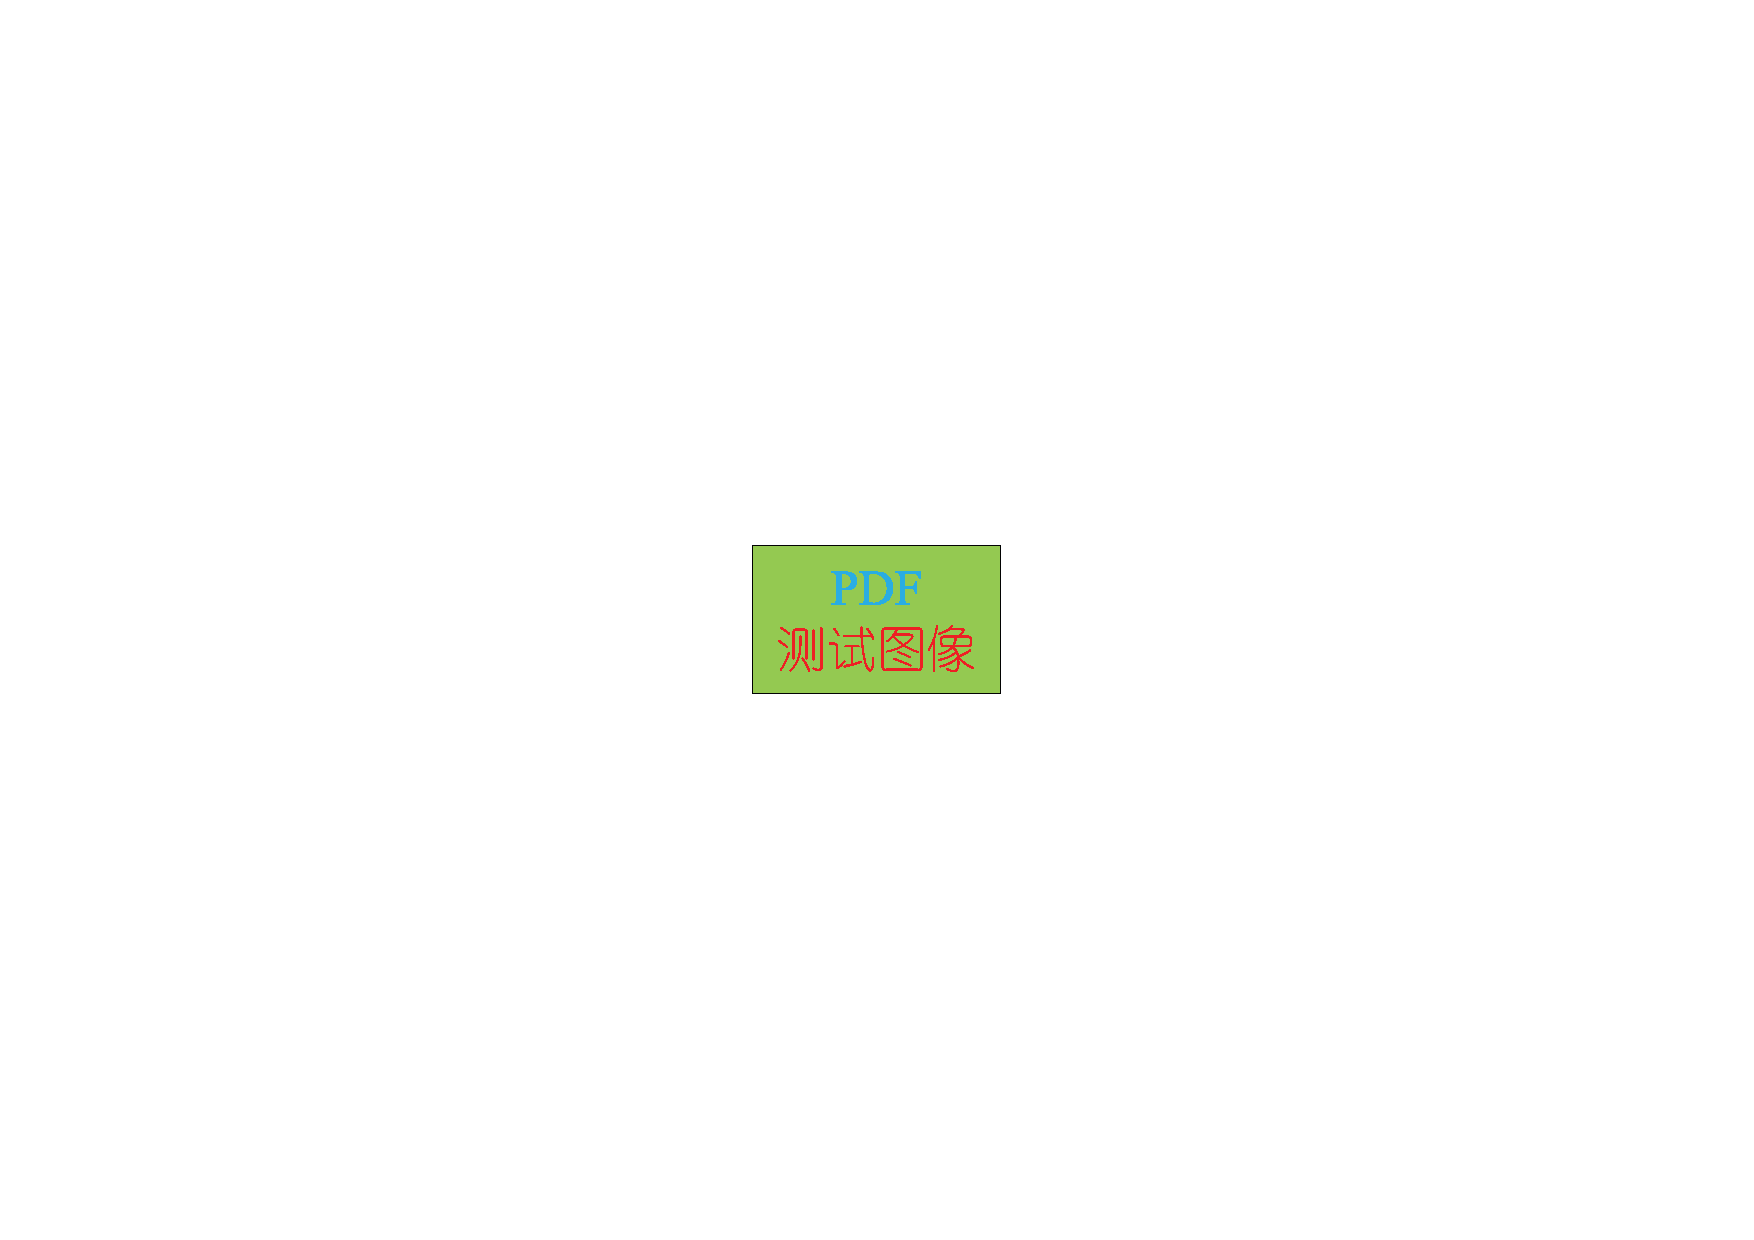
\includegraphics[angle=-90,origin=br,width=4cm]{chap2/testpdf.pdf}
      \bicaption[fig:longcaptiongood]{这里将出现在插图索引}{海交通大学是我国历史最悠久的高等学府之一,是教育部直属、教育部与上海市共建的全国重点大学.}{Fig}{Where there is a will, there is a way.}
    \end{minipage}     
  \end{figure}

  
\section{表格的例子}
\label{sec:tab}

这一节给出的是一些表格的例子,如表\ref{tab:firstone}所示。

\begin{table}[!hpb]
  \centering
  \bicaption[tab:firstone]{指向一个表格的表目录索引}{一个颇为标准的三线表格\footnotemark[1]}{Table}{A Table}
  \begin{tabular}{@{}llr@{}} \toprule
    \multicolumn{2}{c}{Item} \\ \cmidrule(r){1-2}
    Animal & Description & Price (\$)\\ \midrule
    Gnat & per gram & 13.65 \\
    & each & 0.01 \\
    Gnu & stuffed & 92.50 \\
    Emu & stuffed & 33.33 \\
    Armadillo & frozen & 8.99 \\ \bottomrule
  \end{tabular}
\end{table}
\footnotetext[1]{这个例子来自\href{http://www.ctan.org/tex-archive/macros/latex/contrib/booktabs/booktabs.pdf}{《Publication quality tables in LATEX》}(booktabs宏包的文档)。这也是一个在表格中使用脚注的例子,请留意与threeparttable实现的效果有何不同。}

下面一个是一个更复杂的表格,用threeparttable实现带有脚注的表格,如表\ref{tab:footnote}。

\begin{table}[!htpb]
  \bicaption[tab:footnote]{出现在表目录的标题}{一个带有脚注的表格的例子}{Table}{A Table with footnotes}
  \centering
  \begin{threeparttable}[b]
     \begin{tabular}{ccd{4}cccc}
      \toprule
      \multirow{2}{6mm}{total}&\multicolumn{2}{c}{20\tnote{1}} & \multicolumn{2}{c}{40} &  \multicolumn{2}{c}{60}\\
      \cmidrule(lr){2-3}\cmidrule(lr){4-5}\cmidrule(lr){6-7}
      &www & k & www & k & www & k \\
      \midrule
      &$\underset{(2.12)}{4.22}$ & 120.0140\tnote{2} & 333.15 & 0.0411 & 444.99 & 0.1387 \\
      &168.6123 & 10.86 & 255.37 & 0.0353 & 376.14 & 0.1058 \\
      &6.761    & 0.007 & 235.37 & 0.0267 & 348.66 & 0.1010 \\
      \bottomrule
    \end{tabular}
    \begin{tablenotes}
    \item [1] the first note.% or \item [a]
    \item [2] the second note.% or \item [b]
    \end{tablenotes}
  \end{threeparttable}
\end{table}

\section{参考文献管理}

参考文献的管理是这个学位论文模板又一个好玩的地方。

\subsection{将参考文献的内容与表现分离}

这个论文模板使用BibTeX处理参考文献,这又是一个``内容''与``表现形式''分离的极好例子
\footnote{当然,你也可以手动编参考文献item,直接插入文档中。但是,有BibTeX帮助,我觉得没有人想用这种麻烦的方法,所以就在脚注中说明了。}。
参考文献的``内容''就是reference文件夹下的chap\textit{xx}.bib,参考文献的元数据(名称、作者、出处等)以一定的格式保存在这些纯文本文件中。
.bib文件也可以理解为参考文献的``数据库'',正文中所有引用的参考文件条目都会从这些文件中``析出''。
控制参考文献条目``表现形式''(格式)的是.bst文件。.bst文件定义了参考文献风格,使用不同的参考文献风格能将同一个参考文献条目输出成不同的格式。
当然,一个文档只能使用一个参考文献风格。
按照教务处的要求,本模板使用的是国标GBT7714风格的参考文献。

BibTeX的工作过程是这样的:
BibTeX读取.aux(第一次运行latex得到的)看看你引用了什么参考文献条目,
然后到.bib中找相关条目的信息,
最后根据.bst的格式要求将参考文献条目格式化输出,写到.bbl文件中。
在运行latex将.bbl插入文档之前,你可以用文本编辑器打开它,做一些小的修改。
你会发现,.bbl的格式和你自己手动写item很相似,它已经被赋予了一定的``表现形式''。

.bib数据库中的参考文献条目可以手动编写,也可以在google的学术搜索中找到。
各大数据库\footnote{应该说是国际知名数据库,譬如SCOPUS, IEEE, OSA等,国内数据库在搜索、导出方面一直是差得一塌糊涂。}也支持将参考文献信息导出为.bib,
省时省力。
以Google学术搜索为例:进入\url{http://scholar.google.com},在``学术搜索设置''中,将``文献管理软件''设为``显示导入BibTeX''的连接,保存退出。
然后学术搜索找到文献下会有``导出到BibTeX''连接,点击后Firefox会打开新的标签页,出现类似代码\ref{googlescholar}所示的内容
\footnote{展示这些.bib条目使用了listings宏包,因为listings宏包协调中文的能力很糟糕,所以读者在查看模板的这部分源代码时会看到一些非常麻烦的东西。并且,直接将源代码的这部分内容复制到.bib中可能还会出错。我的建议是:这部分内容留意PDF就足够了。}。
请注意,这个条目离``规范''还有一些距离。

  \begin{lstlisting}[caption={从Google Scholar找到的,但并不规范的.bib条目}, label=googlescholar, float, escapeinside="", numbers=none]
    @phdthesis{"白2008信用风险传染模型和信用衍生品的定价",
      title={{"信用风险传染模型和信用衍生品的定价"}},
      author={"白云芬"},
      year={2008},
      school={"上海交通大学"}
    } 
  \end{lstlisting}

  上面的.bib条目的``名字''\cndash{}``白2008信用风险传染模型和信用衍生品的定价'',包含ASCII以外的字符,BibTeX无法处理;
  条目还缺少了address域,这样编译出来的结果会出现``地址不详'';
  并且,条目还缺少language域,BibTeX需要language域来判断是否是中文参考文献。
  将上面的条目修正(改英文名、增加address和language域),复制到本地的.bib文件中就可以了。
  显然,这里描述的是参考文献的内容,而不是表现形式。

  \begin{lstlisting}[caption={一个符合规范的.bib条目}, label=itemok, float, escapeinside="", numbers=none]
    @phdthesis{bai2008,
      title={{"信用风险传染模型和信用衍生品的定价"}},
      author={"白云芬"},
      year={2008},
      language={zh},
      address={"上海"},
      school={"上海交通大学"}
    } 
  \end{lstlisting}

由于中英文参考文献处理起来有差异,所以需要在参考文献中标注是否是中文文献。
确切地说,BibTeX并不具有区分中英文参考文献的``智能'',这种智慧的来源是.bst文——它定义了处理参考文献的规则。
GBT7714-2005NLang.bst中规定:.bib中的条目,如果条目的``language''域非空,就被认为是中文文献,否则被认为是英文文献。
例如,刚才的文献,就会被认为是中文参考文献,采取一些针对中文的处理方式。

最后,这个条目被bibtex处理后,赋予了一定的``表现形式'',在.bbl文件中以下面的样子出现。
你还可以对它进行小的修改,这是一种很折磨人的终极修改方法。
再次运行latex之后,它将被插入到文档中。

\begin{lstlisting}[caption={.bbl中被格式化之后的条目}, escapeinside="", numbers=none]
\bibitem["白云芬(2008)"]{bai2008}
  \textsc{"白云芬"}.
  \newblock {"信用风险传染模型和信用衍生品的定价"}[D].
  \newblock "上海: 上海交通大学, 2008."
\end{lstlisting}

再罗嗦两句,
.bst文件书写起来非常繁杂\footnote{可以参考\href{http://ftp.ctex.org/mirrors/CTAN/info/bibtex/tamethebeast/ttb_en.pdf}{《Tame The BeaST》}。},书写符合GBT7714标准的.bst文件更是一项浩大的工程。
因此,当大家为漂亮、标准的参考文献列表感到满意时,应该对GBT7714-2005NLang.bst的作者充满谢意。
作者在CTeX BBS发的帖子,请看
\href{http://bbs.ctex.org/viewthread.php?tid=33571&highlight=\%B2\%CE\%BF\%BC\%CE\%C4\%CF\%D7\%2BGB}{文后参考文献著录规则 GB/T 7714-2005}。
关于GB/T 7714-2005标准本身,请看\href{http://bbs.ctex.org/viewthread.php?tid=33571&highlight=GB\%2B\%B2\%CE\%BF\%BC\%CE\%C4\%CF\%D7}{这里}。

再多说两句,.bib是“参考文献的内容”,而控制参考文献表现(格式)的是.bst文件,本模板附带的是GBT7714-2005NLang.bst。

\subsection{在正文中引用参考文献}

参考文献可以分章节管理,只需要在主文件中的参考文献中都包含进去就可以,如\verb+\bibliography{chap1,chap2,...}+。

正文中引用参考文献时,用\verb+\upcite{key1,key2,key3...}+可以产生“上标引用的参考文献”,
如\upcite{Meta_CN,chen2007act,DPMG}。
使用\verb+\cite{key1,key2,key3...}+则可以产生水平引用的参考文献,例如\cite{JohnD,zhubajie,IEEE-1363}。
请看下面的例子,将会穿插使用水平的和上标的参考文献:关于书的\cite{Meta_CN,JohnD,IEEE-1363},关于期刊的\upcite{chen2007act,chen2007ewi},
会议论文\cite{DPMG,kocher99,cnproceed},
硕士学位论文\cite{zhubajie,metamori2004},博士学位论文\upcite{shaheshang,FistSystem01,bai2008},标准文件\cite{IEEE-1363},技术报告\upcite{NPB2},电子文献\cite{xiaoyu2001, CHRISTINE1998},用户手册\cite{RManual}。

最后总结一些注意事项:
\begin{itemize}
\item 参考文献只有在正文中被引用了,才会在最后的参考文献列表中出现;
\item 参考文献``数据库文件''.bib是纯文本文件,请使用UTF-8编码,不要使用GBK编码;
\item 参考文献条目中通过language域是否为空判断是否是中文文献;
\item 参考文献条目同样有“内容”和“表现形式”之分,这种可控性是BibTeX带来的。
\end{itemize}


\subsection{参考文献管理器}

参考文献数据库.bib虽然是纯文本的,可以用任意的文本编辑器查看,但总有人喜欢一个找一个``可视化''地查看每一条参考文献。
我想\href{http://jabref.sourceforge.net/}{JabRef}应该是个很不错的选择。
这是一个Java写的程序,需要JRE才能运行。
就我测试的情况上看,很幸运,JabRef可以顺利打开GBK编码的.bib文件。
但是,打开UTF--8编码的.bib源文件过程中总会崩溃,原因不得而知。
由于我们的.bib文件使用的是UTF-8编码,所以JabRef暂时不可用。

提到参考文献管理器,不得不提到另一个广被使用的软件——\href{http://www.endnote.com/}{EndNote}。
在图书馆的宣讲会上,EndNote被吹得神乎其神,但我发现他对.bib的管理很不友好。
EndNote可以导入.bib文件,却不能导出.bib,只能导出.bbl——被格式化的.bib。
原来,JabRef比较``单纯'',不具备格式化参考文献的能力;
而EndNote有那么一点设置参考文献输出格式的能力,然后就把这种能力滥用,这点搞得我很不爽。
看来,EndNote和Word配合得更好一些。


\section{用listings插入源代码}

原先ctexbook文档类和listings宏包配合使用时,代码在换页时会出现莫名其妙的错误,后来经高人指点,顺利解决了。
感兴趣的话,可以看看\href{http://bbs.ctex.org/viewthread.php?tid=53451}{这里}。
这里给使用listings宏包插入源代码的例子,这里是一段C代码。
另外,listings宏包真可谓博大精深,可以实现各种复杂、漂亮的效果,想要进一步学习的同学,可以参考
\href{http://mirror.ctan.org/macros/latex/contrib/listings/listings.pdf}{listings宏包手册}。

\begin{lstlisting}[language={C}, caption={一段C源代码}]
#include <stdio.h>
#include <unistd.h>
#include <sys/types.h>
#include <sys/wait.h>

int main() {
  pid_t pid;

  switch ((pid = fork())) {
  case -1:
    printf("fork failed\n");
    break;
  case 0:
    /* child calls exec */
    execl("/bin/ls", "ls", "-l", (char*)0);
    printf("execl failed\n");
    break;
  default:
    /* parent uses wait to suspend execution until child finishes */
    wait((int*)0);
    printf("is completed\n");
    break;
  }

  return 0;
}
\end{lstlisting}


%%==================================================
%% chapter03.tex for SJTU Master Thesis
%% Encoding: UTF-8
%%==================================================

\chapter{常见问题}
\label{chap:faq}

{\bfseries{}Q:我是否能够自由使用这份模板?}

A:这份模板以MIT开源许可证发布,请遵循许可证规范。

{\bfseries{}Q:我的论文是Word排版的,学校图书馆是不是只收{\LaTeX}排版的论文?}

A:当然不是,Word版论文肯定收。

{\bfseries{}Q:我的论文是{\LaTeX}排版的,学校图书馆是不是只收Word排版的论文?}

A:当然不是,PDF版的电子论文是可以上交的。是否要交Word版就看你导师的喜好了。

{\bfseries{}Q:为什么屏幕上显示的左右页边距不一样?}

A:模板默认是双面打印,迎面页和背面页的页边距是要交换的,多出来的那一部分是留作装订的。

{\bfseries{}Q:为什么在参考文献中会有“//”符号?}

A:那就是国标GBT7714参考文献风格规定的。

{\bfseries{}Q:为什么参考文献中会有[s.n.],[S.l], [EB/OL]等符号?}

A: 那也是国标GBT7714参考文献风格定义的。[s.n.]表示出版者不祥,[S.l]表示出版地不祥,[EB/OL]表示引用的参考文献类型为在线电子文档。

{\bfseries{}Q:如何获得帮助和反馈意见?}

A:你可以通过\href{https://github.com/weijianwen/sjtu-thesis-template-latex/issues}{在github上开issue}
、在\href{https://bbs.sjtu.edu.cn/bbsdoc?board=TeX_LaTeX}{水源LaTeX版}发帖反映你使用过程中遇到的问题。

{\bfseries{}Q:使用文本编辑器查看tex文件时遇到乱码?}

A:请确保你的文本编辑器使用UTF-8编码打开了tex源文件。

{\bfseries{}Q:在CTeX编译模板遇到“rsfs10.tfm already exists”的错误提示?}

A:请删除\verb+X:\CTEX\UserData\fonts\tfm\public\rsfs+下的文件再重新编译。问题讨论见\href{https://bbs.sjtu.edu.cn/bbstcon,board,TeX_LaTeX,reid,1352982719.html}{水源2023号帖}。

{\bfseries{}Q:升级了TeXLive 2012,编译后的文档出现“minus”等字样?}

A:这是xltxtra和fontspec宏包导致的问题。学位论文模板从0.5起使用metatlog宏包代替xltxtra生成{\XeTeX}标志,解决了这个问题。

{\bfseries{}Q:为什么在bib中加入的参考文献,没有在参考文献列表中出现?}

A: bib中的参考文献条目,只有通过\verb+\cite+或者\verb+\upcite+在正文中引用,才会加入到参考文献列表中。

{\bfseries{}如何向你致谢?}

A:请在模板的\href{https://github.com/weijianwen/sjtu-thesis-template-latex}{github主页}点击“Star”,我想粗略统计一下使用学位论文模板的人数,谢谢大家。


%%==================================================
%% conclusion.tex for SJTUThesis
%% Encoding: UTF-8
%%==================================================

\begin{summary}

这里是全文总结内容。

2015年2月28日,中央在北京召开全国精神文明建设工作表彰暨学雷锋志愿服务大会,公布全国文明城市(区)、文明村镇、文明单位名单。上海交通大学荣获全国文明单位称号。         

全国文明单位这一荣誉是对交大人始终高度重视文明文化工作的肯定,是对交大长期以来文明创建工作成绩的褒奖。在学校党委、文明委的领导下,交大坚持将文明创建工作纳入学校建设世界一流大学的工作中,全体师生医护员工群策群力、积极开拓,落实国家和上海市有关文明创建的各项要求,以改革创新、科学发展为主线,以质量提升为目标,聚焦文明创建工作出现的重点和难点,优化文明创建工作机制,传播学校良好形象,提升社会美誉度,显著增强学校软实力。2007至2012年间,上海交大连续三届荣获“上海市文明单位”称号,成为创建全国文明单位的新起点。         

上海交大自启动争创全国文明单位工作以来,凝魂聚气、改革创新,积极培育和践行社会主义核心价值观。坚持统筹兼顾、多措并举,将争创全国文明单位与学校各项中心工作紧密结合,着力构建学校文明创建新格局,不断提升师生医护员工文明素养,以“冲击世界一流大学汇聚强大精神动力”为指导思想,以“聚焦改革、多元推进、以评促建、丰富内涵、彰显特色”为工作原则,并由全体校领导群策领衔“党的建设深化、思想教育深入、办学成绩显著、大学文化丰富、校园环境优化、社会责任担当”六大板块共28项重点突破工作,全面展现近年来交大文明创建工作的全貌和成就。         

进入新阶段,学校将继续开拓文明创建工作新格局,不断深化工作理念和工作实践,创新工作载体、丰富活动内涵、凸显创建成效,积极服务于学校各项中心工作和改革发展的大局面,在上级党委、文明委的关心下,在学校党委的直接领导下,与时俱进、开拓创新,为深化内涵建设、加快建成世界一流大学、推动国家进步和社会发展而努力奋斗!       

上海交通大学医学院附属仁济医院也获得全国文明单位称号。      

\end{summary}


\appendix	% 使用英文字母对附录编号,重新定义附录中的公式、图图表编号样式
\renewcommand\theequation{\Alph{chapter}--\arabic{equation}}	
\renewcommand\thefigure{\Alph{chapter}--\arabic{figure}}
\renewcommand\thetable{\Alph{chapter}--\arabic{table}}
\renewcommand\thealgorithm{\Alph{chapter}--\arabic{algorithm}}

%% 附录内容,本科学位论文可以用翻译的文献替代。
%# -*- coding: utf-8-unix -*-
\chapter{搭建模板编译环境}

\section{安装TeX发行版}

\subsection{Mac OS X}

Mac用户可以从MacTeX主页\footnote{\url{https://tug.org/mactex/}}下载最新安装包。
也可以通过brew包管理器\footnote{\url{http://caskroom.io}}安装MacTeX。

\begin{lstlisting}[basicstyle=\small\ttfamily, numbers=none]
brew cask install mactex
\end{lstlisting}

\subsection{RedHat/CentOS}

建议RedHat/CentOS用户使用TeXLive主页\footnote{\url{https://www.tug.org/texlive/}}的脚本来安装TeXLive发行版。
以下命令将把TeXLive发行版安装到当前用户的家目录下。
若计划安装一个供系统上所有用户使用的TeXLive,请使用root账户操作。

\begin{lstlisting}[basicstyle=\small\ttfamily, numbers=none]
wget http://mirror.ctan.org/systems/texlive/tlnet/install-tl-unx.tar.gz
tar xzvpf install-tl-unx.tar.gz
cd install-tl-20150411/
./install-tl
\end{lstlisting}

\subsection{Deepin}

建议Deepin用户使用系统自带的包管理器安装TeXLive发行版:

\begin{lstlisting}[basicstyle=\small\ttfamily, numbers=none]
sudo apt-get install update
sudo apt-get install -y upgrade
sudo apt-get install -y texlive-full
\end{lstlisting}

\section{安装中文字体}

\subsection{Mac OS X}

Mac用户双击字体文件即可安装字体。

\subsection{Linux用户}

Linux用户请先将字体文件复制到字体目录下,调用fc-cache刷新缓存后即可在TeXLive中使用新字体。

\begin{lstlisting}[basicstyle=\small\ttfamily, numbers=none]
mkdir ~/.fonts
cp *.ttf ~/.fonts				# 当前用户可用新字体
cp *.ttf /usr/share/fonts/local/	# 所有用户可以使用新字体
fc-cache -f
\end{lstlisting}


%# -*- coding: utf-8-unix -*-
%% app2.tex for SJTU Master Thesis
%% based on CASthesis
%% modified by wei.jianwen@gmail.com
%% version: 0.3a
%% Encoding: UTF-8
%% last update: Dec 5th, 2010
%%==================================================

\chapter{Maxwell Equations}

选择二维情况,有如下的偏振矢量:
\begin{subequations}
  \begin{eqnarray}
    {\bf E}&=&E_z(r,\theta)\hat{\bf z} \\
    {\bf H}&=&H_r(r,\theta))\hat{ \bf r}+H_\theta(r,\theta)\hat{\bm
      \theta}
  \end{eqnarray}
\end{subequations}
对上式求旋度:
\begin{subequations}
  \begin{eqnarray}
    \nabla\times{\bf E}&=&\frac{1}{r}\frac{\partial E_z}{\partial\theta}{\hat{\bf r}}-\frac{\partial E_z}{\partial r}{\hat{\bm\theta}}\\
    \nabla\times{\bf H}&=&\left[\frac{1}{r}\frac{\partial}{\partial
        r}(rH_\theta)-\frac{1}{r}\frac{\partial
        H_r}{\partial\theta}\right]{\hat{\bf z}}
  \end{eqnarray}
\end{subequations}
因为在柱坐标系下,$\overline{\overline\mu}$是对角的,所以Maxwell方程组中电场$\bf E$的旋度:
\begin{subequations}
  \begin{eqnarray}
    &&\nabla\times{\bf E}=\mathbf{i}\omega{\bf B} \\
    &&\frac{1}{r}\frac{\partial E_z}{\partial\theta}{\hat{\bf
        r}}-\frac{\partial E_z}{\partial
      r}{\hat{\bm\theta}}=\mathbf{i}\omega\mu_rH_r{\hat{\bf r}}+\mathbf{i}\omega\mu_\theta
    H_\theta{\hat{\bm\theta}}
  \end{eqnarray}
\end{subequations}
所以$\bf H$的各个分量可以写为:
\begin{subequations}
  \begin{eqnarray}
    H_r=\frac{1}{\mathbf{i}\omega\mu_r}\frac{1}{r}\frac{\partial
      E_z}{\partial\theta } \\
    H_\theta=-\frac{1}{\mathbf{i}\omega\mu_\theta}\frac{\partial E_z}{\partial r}
  \end{eqnarray}
\end{subequations}
同样地,在柱坐标系下,$\overline{\overline\epsilon}$是对角的,所以Maxwell方程组中磁场$\bf H$的旋度:
\begin{subequations}
  \begin{eqnarray}
    &&\nabla\times{\bf H}=-\mathbf{i}\omega{\bf D}\\
    &&\left[\frac{1}{r}\frac{\partial}{\partial
        r}(rH_\theta)-\frac{1}{r}\frac{\partial
        H_r}{\partial\theta}\right]{\hat{\bf
        z}}=-\mathbf{i}\omega{\overline{\overline\epsilon}}{\bf
      E}=-\mathbf{i}\omega\epsilon_zE_z{\hat{\bf z}} \\
    &&\frac{1}{r}\frac{\partial}{\partial
      r}(rH_\theta)-\frac{1}{r}\frac{\partial
      H_r}{\partial\theta}=-\mathbf{i}\omega\epsilon_zE_z
  \end{eqnarray}
\end{subequations}
由此我们可以得到关于$E_z$的波函数方程:
\begin{eqnarray}
  \frac{1}{\mu_\theta\epsilon_z}\frac{1}{r}\frac{\partial}{\partial r}
  \left(r\frac{\partial E_z}{\partial r}\right)+
  \frac{1}{\mu_r\epsilon_z}\frac{1}{r^2}\frac{\partial^2E_z}{\partial\theta^2}
  +\omega^2 E_z=0
\end{eqnarray}

\chapter{从{\CJKLaTeX}转向{\XeTeX}}
\label{chap:whydvipdfm}

我习惯把v0.2a使用dvipdfmx编译的硕士学位论文模板称为“{\CJKLaTeX}模板”,而这个使用{\XeTeX}引擎(xelatex程序)处理的模板则被称为“{\XeTeX/\LaTeX}模板”。
从{\CJKLaTeX}模板迁移到{\XeTeX\LaTeX}模板的好处有下:
\begin{enumerate}
\item[\large\smiley] 搭建{\XeTeX}环境比搭建{\CJKLaTeX}环境更容易;
\item[\large\smiley] 更简单的字体控制;
\item[\large\smiley] 完美支持PDF/EPS/PNG/JPG图片,不需要“bound box(.bb)”文件;
\item[\large\smiley] 支持OpenType字体的复杂字型变化功能;
\end{enumerate}

当然,这也是有代价的。由于{\XeTeX}比较新,在我看来,使用{\XeTeX}模板所必须付出的代价是:

\begin{enumerate}
\item[\large\frownie] 必须把你“古老的” \TeX 系统更新为较新的版本。TeXLive 2012和CTeX 2.9.2能够编译这份模板,而更早的版本则无能为力。
\item[\large\frownie] 需要花一些时间把你在老模板上的工作迁移到新模板上。
\end{enumerate}

第一条就看你如何取舍了,新系统通常意味着更好的兼容性,值得升级。而转换模板也不是什么特别困难的事情,可以这样完成:

\begin{enumerate}
\item 备份你要转换的源文件,以防你的工作成果丢失;
\item 将你原来的tex以及bib文件另存为UTF-8编码的文件。iconv、vim、emacs、UEdit等等工具都可以完成。WinEdt对文件编码识别功能很差(到了v6.0还是如此),不推荐作为字符编码转换工具;
\item 将diss.tex导言区中的内容替换为XeTeX模板diss.tex导言区的内容;
\item 将你对原先导言区的修改,小心翼翼地合并到新的导言区中;
\item 使用XeTeX模板中的GBT7714-2005NLang.bst替换原有的bst文件,新的bst文件只是将字符编码转换为UTF-8;
\item 删除bouding box文件;
\item 使用本文\ref{sec:process}介绍的方法,重新编译文档;
\end{enumerate}


%%==================================================
%% Encoding: UTF-8
%%==================================================

\chapter{模板更新记录}
\label{chap:updatelog}

\textbf{2015年2月15日} v0.7发布,增加盲审选项,调用外部工具插入扫描件。

\textbf{2015年2月14日} v0.6.5发布,修正一些小问题,缩减git仓库体积,仓库由```sjtu-thesis-template-latex```更名为```SJTUThesis```。

\textbf{2014年12月17日} v0.6发布,学士、硕士、博士学位论文模板合并在了一起。

\textbf{2013年5月26日} v0.5.3发布,更正subsubsection格式错误,这个错误导致如"1.1 小结"这样的标题没有被正确加粗。

\textbf{2012年12月27日} v0.5.2发布,更正拼写错误:从``个人建立''更正为``个人简历''。在diss.tex加入ack.tex,更名后忘了引用。

\textbf{2012年12月21日} v0.5.1发布,在 \LaTeX 命令和中文字符之间留了空格,在Makefile中增加release功能。

\textbf{2012年12月5日} v0.5发布,修改说明文件的措辞,更正Makefile文件,使用metalog宏包替换xltxtra宏包,使用mathtools宏包替换amsmath宏包,移除了所有CJKtilde(\verb+~+)符号。

\textbf{2012年5月30日} v0.4发布,包含交大学士、硕士、博士学位论文模板。模板在\href{https://github.com/weijianwen/sjtu-thesis-template-latex}{github}上管理和更新。

\textbf{2010年12月5日} v0.3a发布,移植到 \XeTeX/\LaTeX 上。

\textbf{2009年12月25日} v0.2a发布,模板由CASthesis改名为sjtumaster。在diss.tex中可以方便地改变正文字号、切换但双面打印。增加了不编号的一章“全文总结”。
添加了可伸缩符号(等号、箭头)的例子,增加了长标题换行的例子。

\textbf{2009年11月20日} v0.1c发布,增加了Linux下使用ctex宏包的注意事项、.bib条目的规范要求,
修正了ctexbook与listings共同使用时的断页错误。

\textbf{2009年11月13日} v0.1b发布,完善了模板使用说明,增加了定理环境、并列子图、三线表格的例子。

\textbf{2009年11月12日} 上海交通大学硕士学位论文 \LaTeX 模板发布,版本0.1a。



\backmatter	% 文后无编号部分 

%% 参考资料
\printbibliography[heading=bibintoc]

%% 致谢、发表论文、申请专利、参与项目、简历
%% 用于盲审的论文需隐去致谢、发表论文、申请专利、参与的项目
\makeatletter
\ifsjtu@review\relax\else
  %%==================================================
%% thanks.tex for SJTU Master Thesis
%% based on CASthesis
%% modified by wei.jianwen@gmail.com
%% version: 0.3a
%% Encoding: UTF-8
%% last update: Dec 5th, 2010
%%==================================================

\begin{thanks}

  感谢所有测试和使用交大学位论文 \LaTeX 模板的同学!

  感谢那位最先制作出博士学位论文 \LaTeX 模板的交大物理系同学!

  感谢~William Wang~同学对模板移植做出的巨大贡献!

\end{thanks}
 	  %% 致谢
  %%==================================================
%% pub.tex for SJTUThesis
%% Encoding: UTF-8
%%==================================================

\begin{publications}{99}
    \item\textsc{Chen H, Chan C~T}. {Acoustic cloaking in three dimensions using acoustic metamaterials}[J]. Applied Physics Letters, 2007, 91:183518.
    \item\textsc{Chen H, Wu B~I, Zhang B}, et al. {Electromagnetic Wave Interactions with a Metamaterial Cloak}[J]. Physical Review Letters, 2007, 99(6):63903.
\end{publications}
	  %% 发表论文
  \begin{patents}{99}
    \item 第一发明人,“永动机”,专利申请号202510149890.0
\end{patents}
	  %% 申请专利
  %# -*- coding: utf-8-unix -*-
%%==================================================
%% projects.tex for SJTUThesis
%% Encoding: UTF-8
%%==================================================

\begin{projects}{99}
    \item 973项目“XXX”
    \item 自然基金项目“XXX”
    \item 国防项目“XXX”
\end{projects}
  %% 参与的项目
% %%==================================================
%% resume.tex for SJTU Master Thesis
%% based on CASthesis
%% modified by wei.jianwen@gmail.com
%% version: 0.3a
%% Encoding: UTF-8
%% last update: Dec 5th, 2010
%%==================================================

\begin{resume}

\begin{resumesection}{基本情况}
xxx,男,上海人,1985 年~12 月出生,未婚,
上海交通大学物理系在读博士研究生。
\end{resumesection}

\begin{resumelist}{教育状况}
XXXX 年~9 月至~XXXX 年~7 月,上海交通大学, 本科,专业:XXXX

XXXX 年~9 月至~XXXX 年~7 月,上海交通大学, 硕士研究生,专业:XXXX

XXXX 年~9 月至~XXXX 年~7 月,上海交通大学,
博士研究生(提前攻读博士),专业:XXXX
\end{resumelist}

\begin{resumelist}{工作经历}
无。
\end{resumelist}

\begin{resumelist}{研究兴趣}
XXXXXXX。
\end{resumelist}

\begin{resumelist}{联系方式}
通讯地址:上海市闵行区东川路800号,上海交通大学物理系

邮编:200240

E-mail: abcde@sjtu.edu.cn
\end{resumelist}

\end{resume}
	  %% 各人简历
\fi
\makeatother

\end{document}
